\chapter{序論}
\label{chap:introduction}

本章では本研究の背景、それを踏まえた上での研究の目的、そして文書の構成について述べる。

\section{研究の背景}
Virtual Reality( VR)の起源は1956年にMorton Heiligによって開発されたSensoramaに遡る。VRとはコンピューターによりシュミレーショ ンされた仮想現実がユーザの動きにインタラクティブに反応することをいう。Sensoramaは視野、音、振動や、香りの刺激による仮想現実体験マシーンだ\cite{sensorama}。日常生活を抜け出して場所や時間の制約を超えて架空の現実を体験することは長い間人類の夢であった\cite{verge}。しかし技術的制約や制作コストが高いという問題があり一般に普及は難しかった。\\

2014年にFacebookがHead Mounted Display(HMD)を開発したOCULUSを買収してからVRの市場は一気に広がった\cite{vrtrendShiny}。HMDとは頭部に装着するディスプレイ装置のことである。そして今は世界中の企業やクリエイターにより3次元のディスプレーシュミレーション空間のが次々に生み出されている。図\ref{trends}は年代別に制作された仮想現実のシュミレーション環境の数を示している\cite{vrtrendSamuel}。\\
\begin{figure}[htbp]
\begin{center}
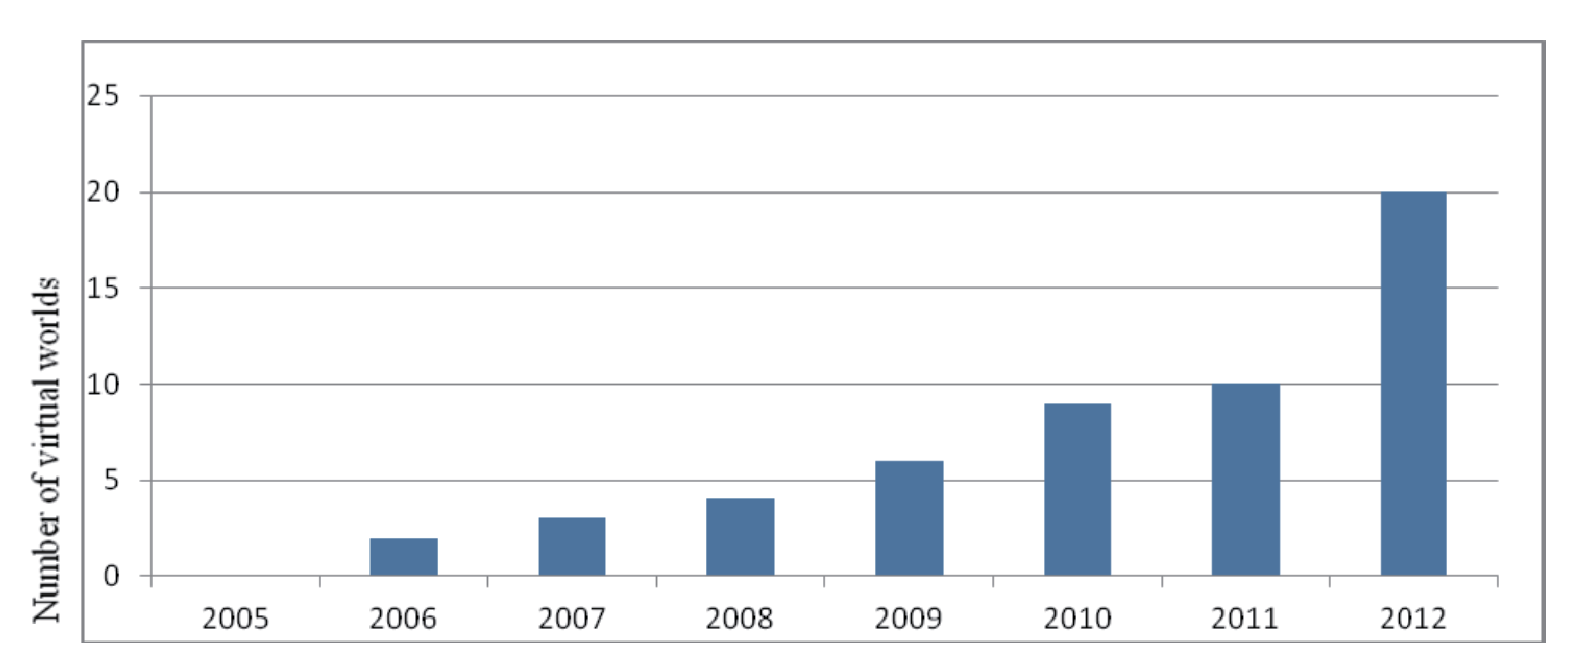
\includegraphics[width=15cm]{eps/vrTrends.eps}
\caption{VirtualRealityのシュミレーション環境の推移}
\label{trends}
\end{center}
\end{figure}

OCULUSは目を完全に覆う没入型の装置で、頭部の動きを3次元トラッキングしてよりインタラクティブでリアルな仮想現実が体験できるようになっている。最近OCULUSはtouchというコントローラーを独自に開発し、仮想空間の中でより直感的な操作を可能にした\cite{touch}。
一方でHTC Viveは70個のセンサーを備え、顔の動きを360度トラッキングできる\cite{vive}。技術はどんどん発展しているがどちらも5万円以上で非常に高額になっている。\\

そこで大衆向けに安価な価格で開発され発売されるようになったのが、Samsung's Gear VR headsetである\cite{samsung}。セッティングも一般ユーザーのために簡単になった。他にもダンボールで作られているGoogleのCardBoardがある。こちらはiPhoneを3Dディスプレーとして使うため2000円で購入が可能である。Cardboard用のアプリの数も増えていて、販売後1ヶ月で1万人が使うようになった\cite{cardboard}。ところがスマートフォンによるVR体験のほとんどはコンサートやローラーコースター、美術館の体験などが多くインタラクティブなものは少ない。\\

またHMDには幾つかの技術的制約があるとOculous VR共同創立者のNate Mitchellが述べている\cite{oculus}。例えば一人称の仮想空間の場合体験者に違和感を感じさせないために身長をユーザーと一致させることで目線を合わせたり、自身の手や足などを拡張空間の中でも作り上げるために全身のトラッキングシステムを考えなかればならない。また物体や空間をよりリアルに見せるために影、テキスタイル、動き、重力や音を正確に表現しなければならならない\cite{vrtrendShiny}。そしてユーザーが乗り物酔いのようにするためには1秒に75フレームのスピードでレンダリングを行わなければならい\cite{HMDifficulties}。UNITYというゲームエンジンなどを使うことでそれらの作業は比較的楽になったがVRコンテンツ制作には声優、デザイナー、アーティストやエンジニアが必要になる。そのためヘッドマウントディスプレーによる仮想空間は多数向けのコンテンツに留まっている。\\

例えば物理的壁を越えて遠くにいる人と会いたい、時間的壁を越えて過去に旅行をした時の思い出を再び体験したい、自ら好きな映画の登場人物となって刺激を感じてみたいと思っても、その人のモデリングデータをまず入力しなければならない。エンジニアリングの知識のないユーザーにとってそういったパーソナルなコンテンツの作成はできないのだ。\\

そこで本研究では新たな種類の仮想現実を体験するための新しい手法として、明晰夢(睡眠中にみる夢のうち自分で夢を見ていることを自覚していながら見ている夢)に着目した。意識することは少ないが人は毎晩睡眠中に人々は仮想現実を体験している。辞書 『大辞泉 第二版』によると、夢とは「睡眠中にあたかも現実の経験であるかのように感じる一連の観念や心像のこと」\cite{dream}と書かれている。\\

明晰夢は1867 年に Saint Denys により研究が行われて以来\cite{saintDenys}、心理学者や哲学者の間で研究が進められてきた。明晰夢の経験者は夢の状況を自分の思い通りに変化させられる、言い換えれば仮想現実を体験することができると語られてきた。 スタンフォード大学博士の Stephen LaBergeは1987 年に The Lucidity Institute を設立し、明晰夢を見るためのステッ プを Mnemonic Induction of Lucid Dreams (The MILD Technique) で紹介した\cite{LaBerge}。しかしThe MILD Techniqueを習得するには特殊な訓練が必要だ。例えば就寝してから5時間たつときにアラームをかけて一度起きて、明晰夢のことを念じながらもう一度寝る。また明晰夢を見るためには、夢を見ているか否かを自覚できる体質にならなければならない。そのためにリアリティーチェックといって、起床中も夢を見ているのか否かを確認する習慣を付けておく必要がある。例えば夢の本数が正確であるかを確認する、口と鼻から息をしっかりしているか確認する、あるいは鏡に覗き込み自分が映るか確認する、ジャンプをして重力を感じるか試すなど、方法は個人によって様々である。他にも夢日記を欠かさず付けて普段から夢を覚えている体質になること。眠りにつく前に体制を正して、深呼吸をし心を落ち着かせる。そして「これから明晰夢を見るんだ」と念じならが寝る。夢で見たい内容を思い浮かべる。MILDは労力が必要で誰もが気軽に始められるものとは言い難い。

\section{研究の目的}
ユーザーの思い出から特定の人物や空間をVRで登場させることはHMDでは難しかった。だからこそ本研究ではHMDに変わって明晰夢に着目する。特別な訓練をしなくても明晰夢を実現できる新しい手法として、レム睡眠・ノ ンレム睡眠かを観測し起きる直前のレム睡眠中にユーザが望む体験に関連のある音を流すスマー トフォンアプリケーションである DreameDate を開発する。\\

明晰夢を促進するデバイスとしては株式会社タカラトミーが開発した夢見工房\cite{takaratomi}やDreamON\cite{dreamOn}などのスマートフォンアプリが提案されているが、どれも商業目的のものが多く信頼性の高い実験データを公開していないため有効性については大いに疑問が残る。そこでDreamDateでは具体的に以下の点を検証したい。

\begin{itemize}
\item 検証1:夢を操作するために効果的な外的刺激の種類
\item 検証2:外的刺激の与え方とタイミング
\item 検証3:ユーザーに精神的・金銭的負担のかからない睡眠観測方法について
\item 検証4:明晰夢を通して仮想現実を体験できるか
\end{itemize}

人生の1/3を過ごす睡眠時間をより有効的に使うことができれば人類の発展に大いに繋がる。これまでにない新しい睡眠のスタイルの実現に貢献したい。

\section{本文書の構成}
第\ref{chap:introduction}章では、本論文を書くに至った背景と目的、そして論文の構成を説明している。第\ref{chap:webapi}章ではユーザーの仮想現実や明晰夢における認識度や要求について事前調査、睡眠中に見る夢の分析を行った。また睡眠観測や明晰夢促進という目線での先行研究や開発事例を述べたのちに、複数の 観点からDreamDateとの比較を行い新しい解決方法について提起する。第\ref{chap:search}章ではDreamDateのプロトタイピングの過程と、システムの概要、利用方法について述べる。第\ref{chap:visualize}章では章では本研究で試作した DreamDateのユーザースタディの結果と考察を述べる。第\ref{chap:coding}章では本研究の総括を行い、また今後の展望について議論する。最後に備考を述べる。
